\chapter{Space Plug-and-Play Architecture}\label{ch:spa}
Space plug-and-play Architecture (SPA) is a set of standards that define how
different players can create plug-and-play components that can easily be
assembled to form a complete satellite for a specific mission. The standards
are published by American Institute of Aeronatuics and Astronautics (AIAA). The
standards range from how power supply should be handled to how components
communicate in the application layer, focus in this report is put on the
software parts.

To describe how a SPA network works some terminology needs to be defined. All
nodes in a SPA network are called "components", there is no differentiation
between software and hardware components. Each component has a "Component
Universally Unique Identifier" (CUUID) which is 128 bit long. Each component
also has an "Extensible Transducer Electronic Data Sheet" (xTEDS) file that
describes respective components capabilities. To be able to support different
underlying link layer technologies such as Ethernet, Spacewire and one-wire
(I2C), most functionality has been put in the application layer. This means
that a SPA network can be built with any combination of link layer "subnets",
for example a SPA network can consist of two Spacewire subnets and one Ethernet
subnet.

\nomenclature{\textbf{CUUID}}{\textbf{Component Universally Unique Identifier}}

The important concepts to remember is that each SPA component is
connected to one or more SPA subnets, on each SPA subnet there is a subnet
manager (SM-x) that acts as a gateway to other SPA subnets and when SPA subnets
are linked together they form a SPA network. To make things clear, a single SPA
subnet with a CAS, LS and SM-x is also a SPA network.

Another SPA subnet is the SPA Local Subnet. Each processing node that can
have multiple SPA components running on it has a "SPA Local Subnet Manager"
(SM-L).  Components within a processing node should do inter-process
communication over UDP/IP \cite{spa:local-subnet}.

Components communicate with each other with the help of "logical addresses"
that each component recieves during boot up. It is the responsiblity of the
"Central Addressing Service" (CAS) to hand out logical addresses to all
components in the SPA network through the connected Subnet Managers. After a
component receives its logical address it can share its xTEDS file with other
components. It is the responsibility of the "Lookup Service" to keep track of
the capabilities of each component in the SPA network.

To describe what a SPA network can look like figure
\ref{fig:minimal_spa_network} shows a minimal SPA network which consists of a
CAS, LS, a sensor and a monitor application, all running on the same processing
node and in the same local subnet managed by the SM-L.

\begin{figure}[h]
    \centering
    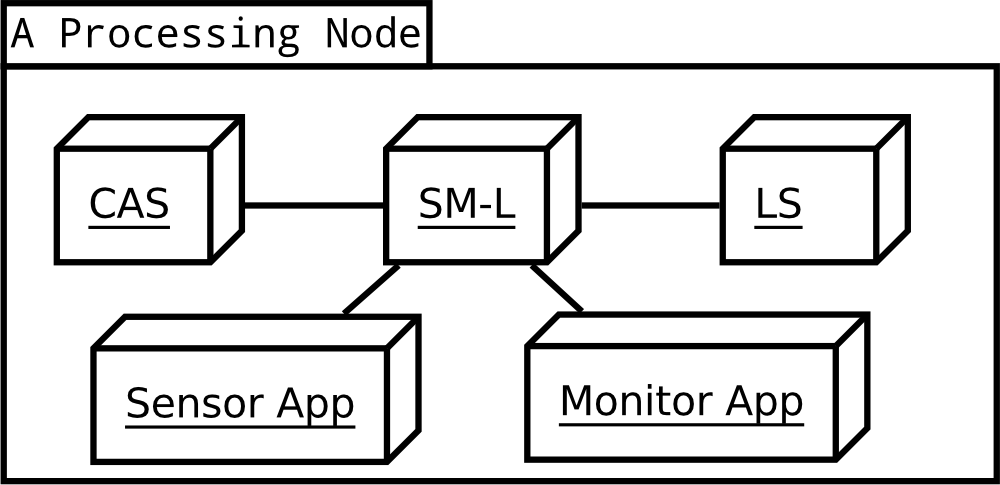
\includegraphics[width=\textwidth]{figures/minimal_spa_network}
    \caption{A processing node running a minimal SPA network.}
    \label{fig:minimal_spa_network}
\end{figure}

A more complex SPA network is shown in figure \ref{fig:complex_spa_network}.
Three different processing nodes are connceted to each other over a
SPA-Ethernet subnet. The CAS, LS and Monitor Application are now running on
different nodes and the sensor application is located on its own embedded
device.

\begin{figure}[h]
    \centering
    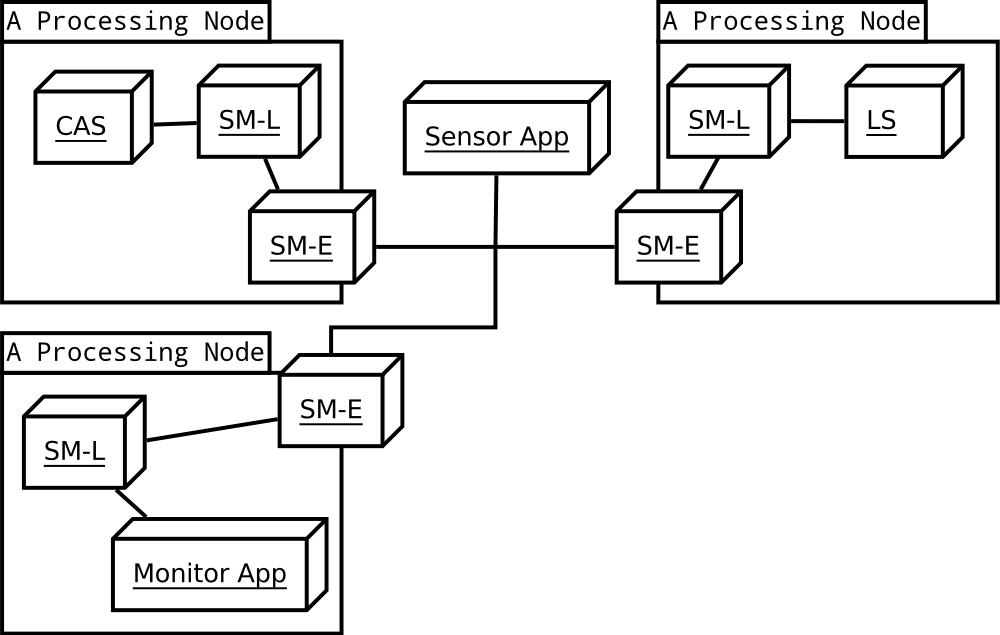
\includegraphics[width=\textwidth]{figures/complex_spa_network}
    \caption{A SPA network with multiple subnets.}
    \label{fig:complex_spa_network}
\end{figure}

For a detailed view on how SPA works the SPA standards is the best source for
information. The SPA standards and drafts that specify software requirements
are the Logical Interface standard \cite{spa:logical-interface}, Networking
standard \cite{spa:networking}, Local Subnet Draft \cite{spa:local-subnet},
Ontology Standard \cite{spa:ontology} and System Capabilities Standard
\cite{spa:system-capabilities}.


% \section{Virtual Network and the Virtual Network Protocol}
% TODO: Finish of with the definition of Virtual Network, Virtual Network
% Protocol and how it relates to SPA.
%
% TODO: Is this needed or should VNP perhaps only be mentioned in context with
% development efforts and code? This would mean that all comments about VN/VNP is
% pushed to the results and conclusion parts...perhaps some in the method.
